% !TeX root = ../../../main.tex

Finally, we compare partonic luminosities and \lhc differential distributions
obtained with \nnpdfr{4.0} in \cref{sec:afb/largexpdfs} and \cref{sec:afb/afb}
with those based  on its predecessor \nnpdfr{3.1}, as well as with a variant of
\nnpdfr{4.0} where positivity is imposed at the level of observable
cross-sections but not at the \pdf level, as was the case in  \nnpdfr{3.1}, which
we will denote \nnpdfr{4.0}(3.1pos).

\Cref{fig:afb/pdfplot-absDYlumis-pdfsets-plus-q5tev-nnpdf31} compares the 
symmetric partonic luminosities $\mathcal{L}_{S,q}$ evaluated for
$\mll=\SI{5}{\tera\electronvolt}$.
%
The three sets are found to agree within uncertainties,
with \nnpdfr{4.0} having the smallest uncertainties.
%
This increase in precision arises only marginally due to the more restrictive
positivity constraints imposed, since predictions with the \nnpdfr{4.0}(3.1pos)
variant  are close to the baseline \nnpdfr{4.0}, especially  for the $u\bar{u}$
contribution, for both central values and uncertainties.
%
The comparison in \cref{fig:afb/pdfplot-absDYlumis-pdfsets-plus-q5tev-nnpdf31}
indicates that phenomenological predictions for high-mass \acrlong{dy}
production based on \nnpdfr{3.1} are expected
to be consistent within errors with those of \nnpdfr{4.0} for the contributions
symmetric in $\cos\theta^*$, such as the $|\yll|$ distribution.

%-------------------------------------------------------------------------------
\begin{figure}[!t]
 \centering
 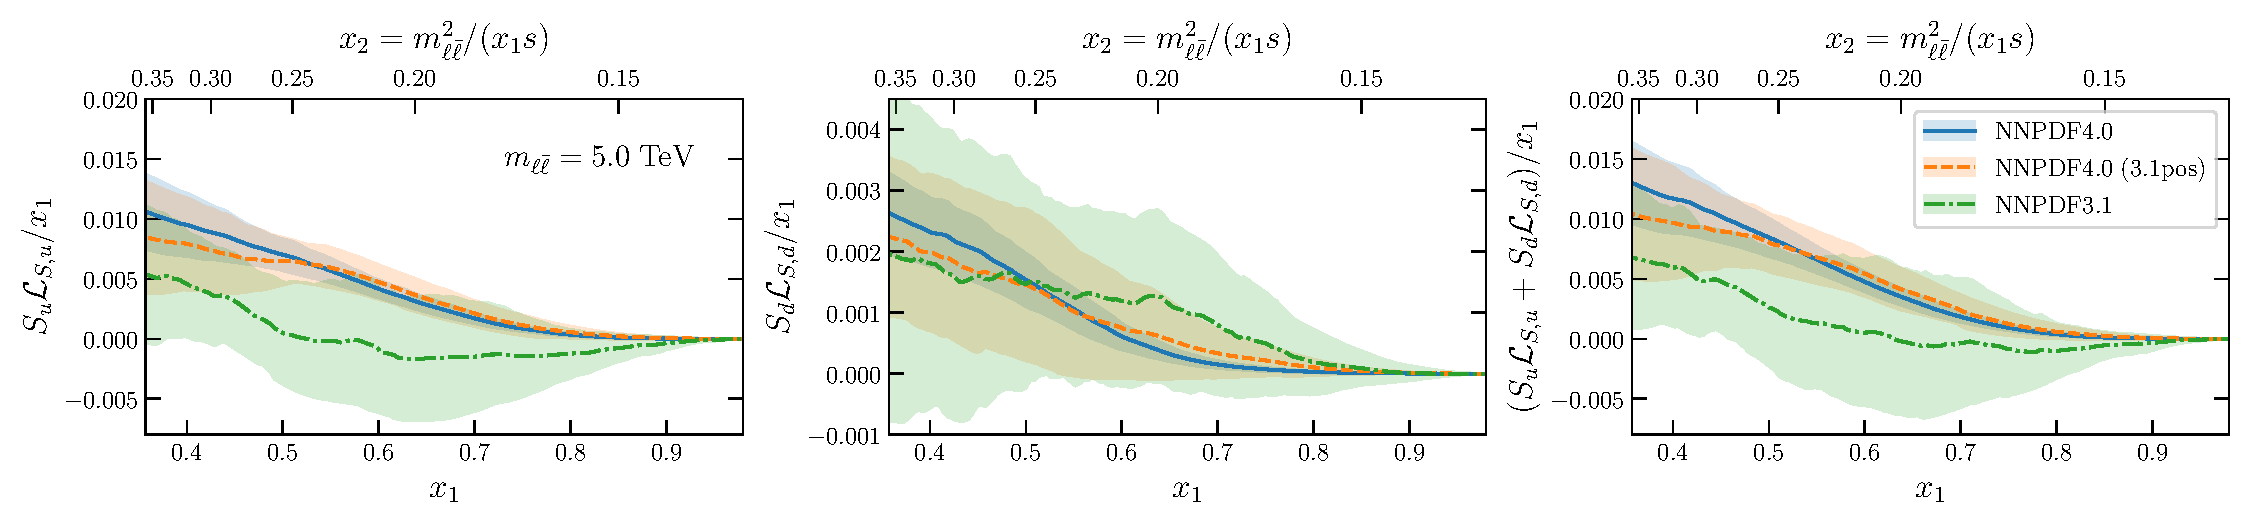
\includegraphics[width=0.99\linewidth]{ch-afb/pdfplot-abs-jacobian-DYlumis-pdfsets-plus-q5p0tev-nnpdf31.pdf}
 \caption{Same as \cref{fig:afb/mll_dep_lumi_plus} (upper panels) comparing
\nnpdfr{4.0}, \nnpdfr{4.0}(3.1pos), and \nnpdfr{3.1}.
 }    
 \label{fig:afb/pdfplot-absDYlumis-pdfsets-plus-q5tev-nnpdf31}
\end{figure}
%---------------------------------------------------------------------------

The antisymmetric luminosities $\mathcal{L}_{A,q}$, relevant for the
forward-backward asymmetry, are displayed in \cref{fig:afb/pdfplot-absDYlumis-pdfsets-minus-q5tev-nnpdf31}
for $\mll = 3$ and 5 TeV respectively.
%
Their qualitative behavior is similar for all  \pdf sets,
with a marked decrease of \pdf uncertainties first from \nnpdfr{3.1}
to  \nnpdfr{4.0}(3.1pos)  then
to \nnpdfr{4.0}.
%
Specifically, the qualitative $\mll$ dependence
of $\mathcal{L}_{A,q}$ remains unchanged. Namely, the positive $A_{\text{fb}}$
found for $\mll= \SI{3}{\tera\electronvolt}$ decreases 
as the dilepton invariant mass is increased.
%
Hence also for the component of the \acrlong{dy} cross-section which is odd
in $\cos\theta^*$ we expect \lhc predictions based on \nnpdfr{3.1} to be consistent
with those obtained from \nnpdfr{4.0}.

%-------------------------------------------------------------------------------
\begin{figure}[!t]
 \centering
 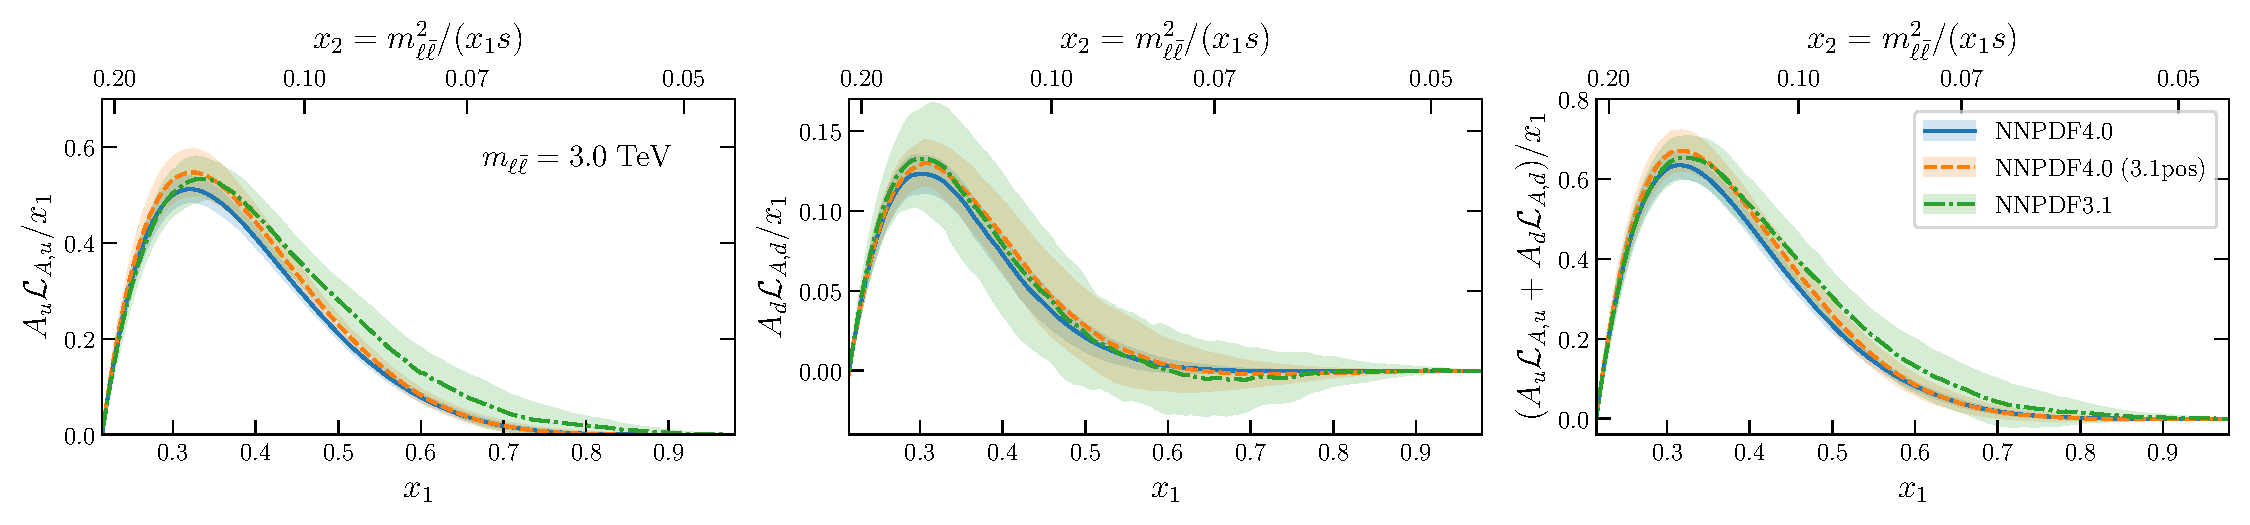
\includegraphics[width=0.99\linewidth]{ch-afb/pdfplot-abs-jacobian-DYlumis-pdfsets-minus-q3p0tev-nnpdf31.pdf}
 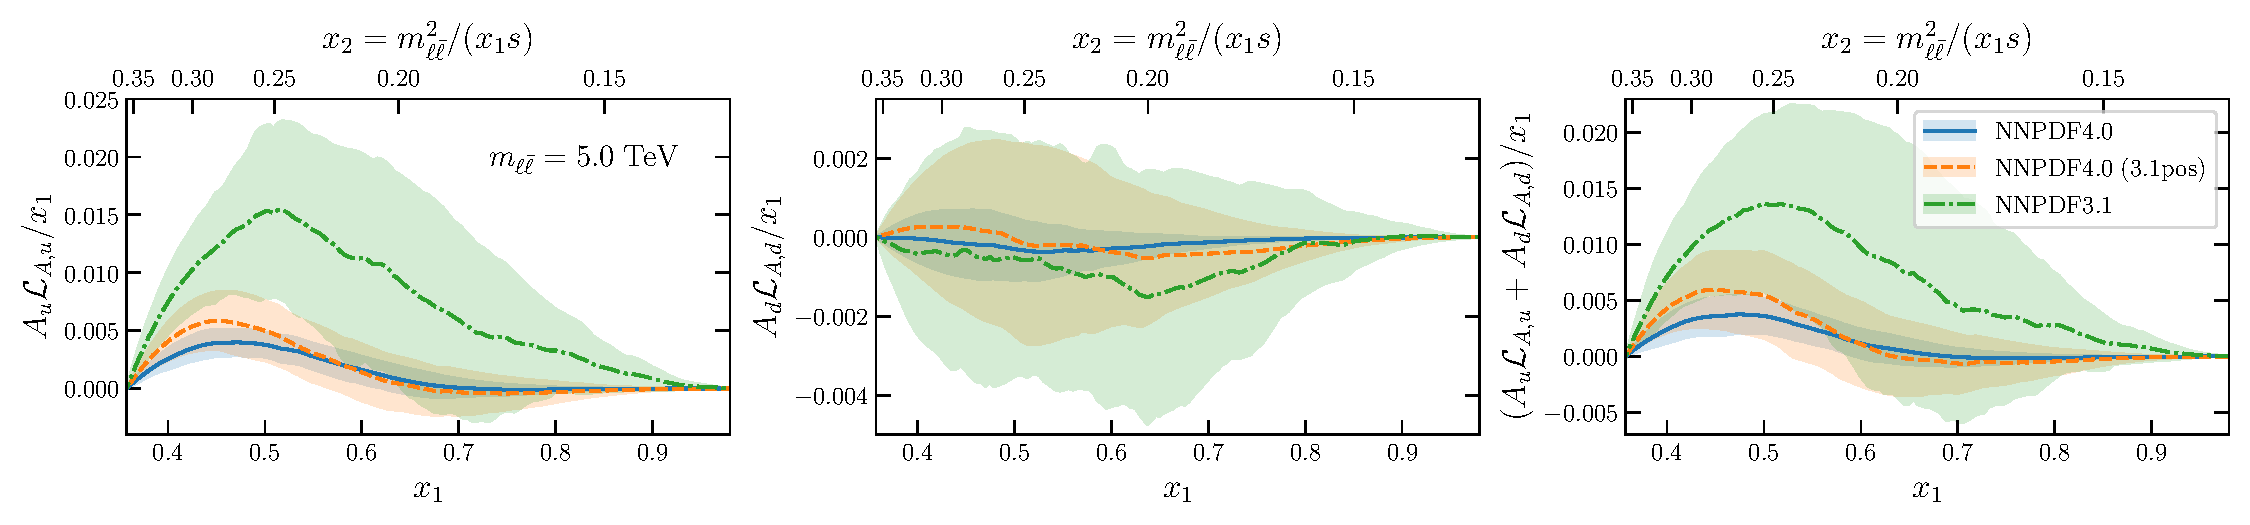
\includegraphics[width=0.99\linewidth]{ch-afb/pdfplot-abs-jacobian-DYlumis-pdfsets-minus-q5p0tev-nnpdf31.pdf}
 \caption{Same as \cref{fig:afb/mll_dep_lumi_minus} for the antisymmetric partonic luminosities $\mathcal{L}_{A,q}$,
   comparing \nnpdfr{4.0}, \nnpdfr{4.0}(3.1pos), and \nnpdfr{3.1}.
 }    
 \label{fig:afb/pdfplot-absDYlumis-pdfsets-minus-q5tev-nnpdf31}
\end{figure}
%---------------------------------------------------------------------------

These expectations are confirmed by
\cref{fig:afb/CMS_DY_14TEV_COSTH_5000_YLL40-vs-31}, which shows the
dilepton rapidity $|y_{\ell\bar{\ell}}|$ 
and the \acrlong{cs} angle $\cos\theta^*$ distributions for neutral-current DY production
at the \lhc 14 TeV for dilepton invariant masses of $m_{\ell\bar{\ell}}\ge \SI{5}{\tera\electronvolt}$,
comparing the baseline \nnpdfr{4.0} predictions with those from \nnpdfr{3.1}
and \nnpdfr{4.0}(3.1pos).
%
Indeed, 
good agreement within the three \pdf sets is observed with a significant reduction
of \pdf uncertainties between \nnpdfr{3.1} and \nnpdfr{4.0}, consistent
with the behaviour exhibited by the corresponding partonic luminosities.

%-------------------------------------------------------------------------------
\begin{figure}[!t]
 \centering
 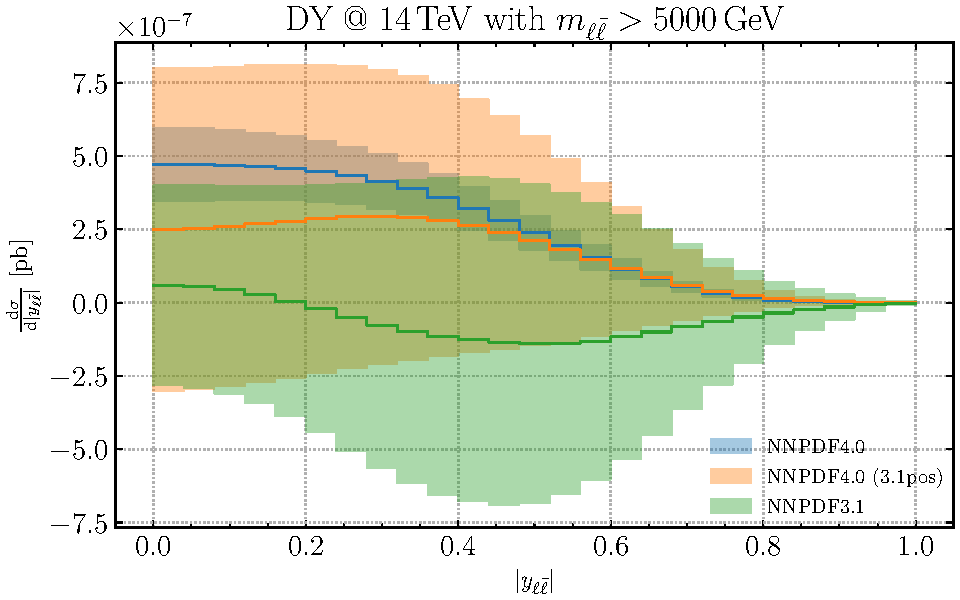
\includegraphics[width=0.49\linewidth]{ch-afb/NNPDF_DY_14TEV_BSM_AFB_YLL_5000-40-vs-31}
 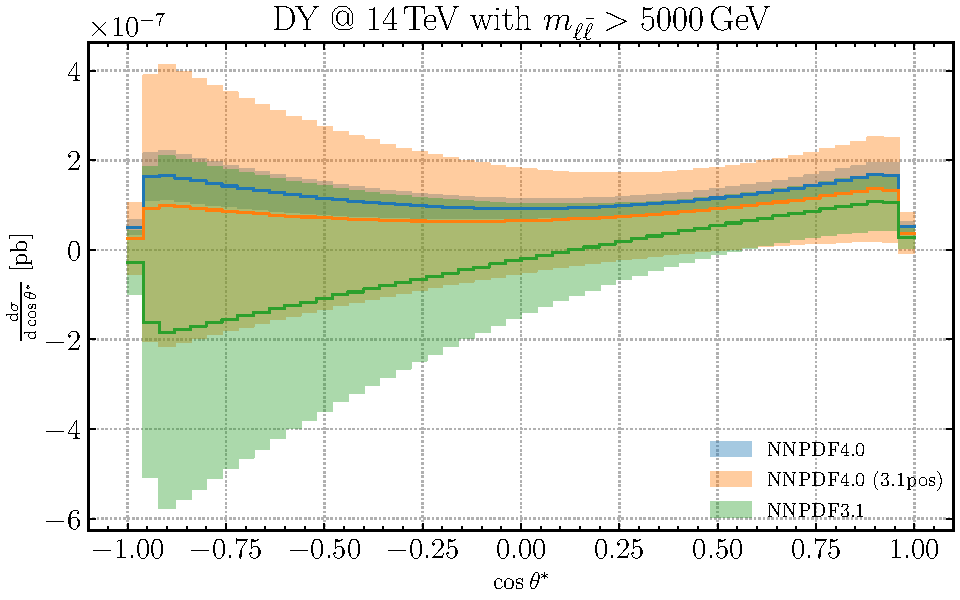
\includegraphics[width=0.49\linewidth]{ch-afb/NNPDF_DY_14TEV_BSM_AFB_COS_5000-40-vs-31}
 \caption{
   Same as
   \cref{fig:afb/CMS_DY_14TEV_MLL_5000_rap,fig:afb/CMS_DY_14TEV_MLL_others} for
   the absolute dilepton rapidity $|y_{\ell\bar{\ell}}|$ (left) and the $\cos
   \theta^*$ (right) distributions for dilepton invariant masses of
   $m_{\ell\bar{\ell}}\ge \SI{5}{\tera\electronvolt}$ comparing \nnpdfr{4.0},
   \nnpdfr{4.0}(3.1pos), and \nnpdfr{3.1}.
 }    
 \label{fig:afb/CMS_DY_14TEV_COSTH_5000_YLL40-vs-31}
\end{figure}
%---------------------------------------------------------------------------
